\section{System}

%In this section, we first give an overview of our system
%for relation schema inferring,
%then we present the detail of each step in the system.
%%\KZ{Avoid the name RvSp, just say the system, or our system. Replace all
%%specific mentions of Freebase by more generic notion. This is possible
%%given that you have done the formal problem definition.}
%
%
%\subsection{System Overview}
% 3 main work: entity linking, relation merging, sel. pref.

\begin{figure*}[htp]
\centering \scalebox{0.65}{\includegraphics[angle=270]{system-crop.eps}}
%\epsfig{file=figure1-cropped.eps, width=2\columnwidth}
%\scalebox{0.35}
\caption{System Architecture}
\label{fig:workflow}
\end{figure*}
%\KZ{Redraw this figure as the three boxes in the middle turned out to be
%black in my version of PDF. Also, instead of naming ``ReVerb'' and ``Freebase''
%specifically, use generic terms like ``Open IE'' and ``Taxonomy''. We want
%this system to be general and not tied specifically to ReVerb or Freebase,
%though the actual implementation and eval are on ReVerb and Freebase. These
%we can say in the eval section.}

The workflow of our system is shown in Figure \figref{fig:workflow}.
% input: reverb relation, total 3 steps (2 sent)
The system takes Open IE relation tuples as the input,
then performs entity linking, relation grouping and schema ranking
to translate them into final ranked list of schemas.

% firstly, entity linking (3 sent)
{\bf(1) Entity Linking:}
Relation arguments are linked to entities in the knowledge base by
fuzzy string matching. Each entity in the knowledge base has a unique identifier.

% secondly, relation grouping (2 sent)
{\bf(2) Relation Grouping:}
Linked tuples sharing similar relation patterns are grouped together.
Besides, each group has a representative relation pattern, which is generated from all the patterns within the group.

% thirdly, simultaneously SP (3 sent)
% need to refine at the last sentence.
{\bf(3) Schema Ranking:}
For each linked tuple in one relation group, argument entities are transformed into types drawn from the knowledge base.
%The selectional association model considers both types simultaneously, and then produce a list of schemas for the relation group.
Then this procedure ranks type pairs (schemas) in terms of how much Open IE tuples a type pair can cover and how specific a type concept is.

\subsection{Entity Linking}

% 11 sentences

% main: tfidf for words on freebase
% based on overlap sim.
% pseudo code?
%


% 0. what are we going to do ?
% Given a relation tuple, we are going to find representative Freebase entities
% which stand for the arguments.
% 1. Formally definition
In the entity linking step, by matching arguments to entities in the knowledge base,
each relation tuple is transformed into linked tuples,
$ltup=\langle e_1,\ rel,\ e_2 \rangle$, with linking scores.

% 2. ??? Talk about Freebase
% 3. each mid in FB has one or more entity names.
% example, China and PRC.



%Each entity in Freebase has one or more aliases. The default one is the name of this entity.
%For example, the entity \textit{m.02\_286} has the name ``New York City'' and other aliases
%such as ``The Big Apple'' ``NYC'' and ``Empire City''.
% 4. leverage multiple namees to build an invert index.
We aim to support fuzzy matching between arguments and entity aliases,
so we take all the aliases into consideration, and build an inverted index from words to aliases.
% 5. stop word set is used, and use the idf score to weight words.
Different words in one alias cannot be treated equally. Intuitively, a word
is more important if it occurs in fewer aliases ($n$), and vice versa.
Based on the inverted index, we use inverted document frequency score to
approximately model the weight of a word $w$:
\begin{equation}
idf(w)=1\ /\log(|\{n : w \in n\}|)
\end{equation}

Besides, stop words are removed from aliases, treating their idf scores as 0.
% 6. matching rule: intersect >= N - 1, weighted overlap score >= threshold
In order to measure the probability of fuzzy matching from an argument ($a$) to an alias ($n$),
we introduce the weighted overlap score:
\begin{equation}
overlap(a, n) = \frac {\sum\limits_{w \in a \cap n} idf(w)} {\sum\limits_{w \in a \cup n} idf(w)}
\end{equation}

We merge all the aliases of an entity together to producing a similarity score 
of fuzzy matching between an entity and an argument:
\begin{equation}
\begin{aligned}
sim(e, a) = \max\limits_{n \in Alist(e)} overlap(a, n)
\end{aligned}
\end{equation}

% \KQ{TODO: Two Strategies: Just choose the best separately, or FB 2-hop connectable}

In order to control the quality of candidate entities,
for an argument having $m$ words (with stop words removed),
we only keep entities that have at least one alias
matching $m-1$ words in the argument, and have a similarity score larger than a threshold, $\tau$.
% we can tune the threshold
% we can use formula to show the weighted score, that is intersect / union, weighed.
% 7. multiple matching, select the one with best wScore.
% 8. tie breaker: count occurrence in freebase relations.
%if there still has a tie, the most popular entity is selected. The popularity of an entity is calculated
%by counting number of relations it has in Freebase.
With similarity score computed, we generate 10 best entity candidates 
respectively for both the subject and the object of $rel$.

Next, we model the joint similarity score ($F$) of the relation tuple
$\langle a_1,rel,a_2\rangle$ with each entity pair combination $\langle e_1,e_2\rangle$ in two ways.
One is a \textbf{naive method} which only considers the similarity
between arguments and corresponding entities:
\begin{equation} \label{eqn:naive}
\begin{aligned}
F(a_1, e_1, &a_2, e_2, rel) = \\
            &sim(e_1, a_1) \times sim(e_2, a_2).
\end{aligned}
\end{equation}

The other method takes predicate paths between $e_1$ and $e_2$
into consideration.
Let $\vec{w}$ be the word vector of $rel$,
and $\vec{p}$ be a path of predicates connecting $e_1$ and $e_2$ in at most
2 hops. Here we say two entities $e_1$ and $e_2$ are connected in 1 hop,
if there exists a predicate $p$, such that $p(e_1, e_2)$ (or $p(e_2, e_1)$) is in the knowledge base.

Similarly, $e_1$ and $e_2$ are connected in 2 hops,
if there exists two predicates $p_1, p_2$ and a transition entity $e'$,
such that $p_1(e_1, e')$ (or $p_1(e', e_1)$) and $p_2(e', e_2)$ (or $p_2(e_2, e')$) are in the knowledge base.
 
We hence define the relatedness between $\vec{p}$ and $\vec{w}$ 
in the form of a conditional probability according to the Naive Bayes model:
\begin{equation}
\begin{aligned}
    P(\vec{p}\, |\, \vec{w}) & \approx \prod\nolimits_p P(p\, |\, \vec{w})  \\
                        & \propto \prod\nolimits_p P(p) \prod\nolimits_w P(w\, |\, p),
\end{aligned}
\end{equation}
\noindent
and we follow the IBM alignment Model 1~\cite{yao2014information} to calculate the conditional probability
between predicates and relation words $P(\vec{p}\, |\, \vec{w})$.
Based on the information above, we define a richer joint similarity score, 
considering all valid
paths between $e_1$ and $e_2$:
\begin{equation} \label{eqn:full}
\begin{aligned}
F(a_1, e_1,a_2,&e_2,rel) = sim(e_1,\, a_1) \times\\
               &sim(e_2,\, a_2) \times
		\sum\nolimits_{\vec{p}} P(\vec{p}\,| \vec{w}).
\end{aligned}
\end{equation}

Due to the multiplications, the value of $P(\vec{p}\,| \vec{w})$ varies a lot 
among different entity pair candidates. The large deviation makes 
$P(\vec{p}\,| \vec{w})$ the most important term in \eqnref{eqn:full}, 
especially in the case when none of predicate paths
are similar enough to the relation words.
Therefore, we trust the factor of $P(\vec{p}\,| \vec{w})$ only when 
there exists a similar predicate path.
In practice, we use a threshold $\rho$ to control whether to 
use \eqnref{eqn:full} or \eqnref{eqn:naive}.
We call this an \textbf{ensemble method}.
For each case of entity linking, if there exists one candidate entity pair satisfying $P(\vec{p}\, |\, \vec{w}) > \rho$,
we use the ensemble method, otherwise we fall back to the naive method for the current case.

%\footnote{The popularity of an entity is calculated by counting number of relations it has in the taxonomy.}
%The other strategy (SIM) selects all the $\langle ent1,\ ent2 \rangle$ pairs simultaneously,
%where $ent1$ is reachable from $ent2$ in the taxonomy by 1-hop or 2-hop relation.
%Experimental results on these two strategies are shown in Section 4.


% 9. SUTime is used to map years and datetime.

% check other papers, learn how to introduce FB without too much words.
% 10. discard non-match to guarantee accuracy of linking.
% If one argument fails to link to any entity, the corresponding relation tuple is discarded.
% Ranking Method May Change?
%   use wScore threshold to filter entities
%   then sorting by interLen, then popularity ??? (maybe we can have a try afterwards)
%


%\begin{table}[htbp]
%	\centering
%	\caption{Syntactic Transform Rules}
%	\begin{tabular}{|l|l|}
%		%\toprule
%        \whline
%		Category & Pattern Template \\
%		%\midrule
%        \hline
%        % Continuous Tense & \{$adv_1$\} \textbf{be} \{$adv_2$\} verb:VBG \{text\}
%        %                  & $verb_{lem}$ \{phrase\} \\
%		% Participle Tense & \{$adv_1$\} \textbf{have} \{$adv_2$\} verb:VBN \{text\}
%        %                  & $verb_{lem}$ \{phrase\} \\
%        % Participle + Passive & \{$adv_1$\} \textbf{have} \{$adv_2$\} been \{text\}
%        %                      & is \{text\} \\
%        Continuous Tense & \textbf{be} verb:VBG \{phrase\} \\
%		Participle Tense & \textbf{have} verb:VBN \{text\} \\
%        Future Tense & \textbf{will}/\textbf{shall} verb:VB \{pharse\} \\
%                     & \textbf{be} going to verb:VB \{phrase\} \\
%		%\bottomrule
%        \whline
%	\end{tabular}%
%	\label{tab:synt rules}%
%\end{table}


\subsection{Relation Grouping}
% 8 sents.
% 1. group tuples together, give definition
A relation group consists of a list of linked tuples sharing similar relation patterns,
along with a pattern representing this group, $group(rPat) = \{ltup_1, ltup_2, ..., ltup_k\}$, where
$rPat$ is the representative pattern.
% 2. same & syntactically similar rel. patterns will be in a group, no overlapping.
Each tuple must be contained in only one group.

% 3. algorithm: syntactic rules to convert tense,
% mainly focus on 3 tense: will/should/must be, be -ing, participle
We define syntactically equivalence between two relation patterns, as both of them can be converted
into the same simple pattern by a list of transformations. 
Every relation pattern in one group is equivalent with each other.
Since adverbs and modal verbs are less important
in finding preference of a relation, we firstly remove these words,
and then perform transformation on the remaining relation.
In ReVerb, relations are verb based, the syntactic rules detect different
tenses, such as continuous tense, participle tense, transforming them into present tense.
If the relation has passive voice, it will be kept in the transformed relation.

% 4. Create a table, showing the rules to find them.
%The detail of syntactic rules is shown in Table 1.
%\KQ{refer to Liang et al., 2014 to build the rule table, containing continuous, participle, be-the-name-of
%and passive form}
% For example, a --> b
% check liang's 14 paper to learn the representation of tables.
% 5. use stanford parser to tokenize & postag.
We use Stanford Parser \cite{klein2003accurate} to perform POS tagging, lemmatizing and parsing on relations.
% 6. representative relation: present tense
After transformation, all linked tuples with the same pattern form a group, and this pattern
is selected as representative pattern.


\subsection{Schema Ranking}

Given a relation group, the step of schema ranking produces a ranked list of relation schemas with two constraints.
Take ``play\ in'' as an example, the ideal schemas will contain the pair
$\langle actor,\ film \rangle$ and
$\langle athlete,\ sports\ league \rangle$

Each linked tuple $\langle e_1,\ rel,\ e_2 \rangle$ supports the type pair $\langle t_1,\ t_2 \rangle$
where $(e_1, t_1),\; (e_2, t_2) \in IsA$ in the knowledge base. 
We treat these pairs equally, since it's not trivial to
tell which type is more related to the argument given the relation tuple as context.
Combining all tuples in one group, we define the support of a type pair $tp$
in a group (using the representative pattern $r$ to stand for the group):
\begin{equation}
\begin{aligned}
sup_{r}(&\langle t_1, t_2 \rangle) = \\
        &\{(e_1, t_1) \in IsA,\; (e_2, t_2) \in IsA \}
\end{aligned}
\end{equation}

A simple intuition is to rank schemas by the size of the support.
Since one entity belongs to multiple types, relation schemas with general types
will be ranked higher.
However, two different schemas may share the same support.
For instance, given the relation ``\textit{X die in Y}'', 
suppose Open IE extractions and entity linking step returns correct results,
the schema $\langle person,\ location \rangle$ and $\langle deceased\ person,\ location \rangle$ have identical supports.
The latter one shows a more concrete representation of the relation, because
\textit{deceased person} covers small entities than \textit{person} in the knowledge base.

Therefore, the schemas cannot be ranked by using the support alone.
Next, we aim to extract the subsumption relations between types in the knowledge base,
building the taxonomy of types.

We first define all entities in $t$ as
\begin{equation}
cover(t) = \{e\; |\; (e, t) \in IsA\}.
\end{equation}
Intuitively, type $t_1$ is subsumed in $t_2$, 
if all entities in $t_1$ also belong to $t_2$,
that is, $cover(t_1) \subseteq cover(t_2)$. This uses the idea of
\textbf{strict set inclusion}.
For example, we can learn that the type \textit{person} subsumes types such as
\textit{actor}, \textit{politician} and \textit{deceased person}.

However, strict set inclusion doesn't always hold in the knowledge base.
For example, entities in type \textit{award winner} are mostly \textit{person}, but there still has some
organizations in it. The strict method fails to find the subsumption relation between \textit{award winner}
and \textit{person}, while this subsumption actually holds with a large confidence. 
%
%The ranked list should be adjusted by the IsA relations between the types in
%knowledge base $K$.
%Each type $t$ in $K$ is subsumed by a set of entities (a.k.a. the
%support set). Next we will write $Supp$ to denote the set of entities
%it covers.
%The main difficulty in generating type subsumptions is that the
%support sets may be incomplete \KZ{Why incomplete and isn't type subsumption
%already included in the ISA relation between types?},
%\XS{We can consider ISA relation not explicit between types, thus we need the support set to
%determine the subsumptions between types.}
%thus making strict set inclusion computation impossible.
%\KZ{The rest of this section needs to be rewritten to be consistent
%with the problem definition section. You can't use $S$, which means a set
%of extracted triples, and you can't mention Freebase!}

To resolve this problem, we use a \textbf{relaxed set inclusion},
where the set $cover(t_1)$ can be a subset of another set $cover(t_2)$ to a certain degree.
We define the degree of the subsumption as the ratio between the number 
of entities in the two sets: 
\begin{equation}
deg(t_1 \subseteq t_2) = \frac{\left|cover(t_1) \cap cover(t_2)\right|} {\left|cover(t_1)\right|}.
\end{equation}
%$deg(Supp_1\subseteq Supp_2)=\left|Supp_1 \cap Supp_2\right| / \left|Supp_1\right|$.
If $deg(t_1 \subseteq t_2) > \epsilon$,
then $t_1$ is subsumed by $t_2$, and $\epsilon$ is a confidence parameter 
determined by weight tuning.
By scanning all types in the knowledge base, all subsumption relations 
with enough confidence are extracted, forming our type taxonomy.

With a type hierarchy computed by above relaxed set inclusion, 
we can define a schema 
$\langle t_1,\ t_2\rangle$ subsumes another schema
$\langle t_3,\ t_4\rangle$ if 
i) $t_1$ subsumes $t_3$ and $t_2$ subsumes $t_4$;
ii) $t_1$ subsumes $t_3$ and $t_2 = t_4$; or
iii) $t_2$ subsumes $t_4$ and $t_1 = t_3$.

If a schema (type pair) $tp_1$ subsumes another schema $tp_2$, 
and their supports ($|sup_{r}(tp)|$) are approximately equal, 
we give the more specific schema $tp_2$ a higher rank in the output list.
Here two supports are roughly equal if:
\begin{equation}
\frac{\left|sup_{r}(tp_1)\right|-\left|sup_{r}(tp_2)\right|} {max(\left|sup_{r}(tp_1)\right|,\ \left|sup_{r}(tp_2)\right|)} < \lambda
\end{equation}
\noindent
Where $\lambda$ is a threshold determined in the experiments.

